\documentclass[8pt]{article}
\usepackage[french]{babel}
\usepackage[utf8]{inputenc}
\usepackage[T1]{fontenc} % allows to copy accented words on PDF
\usepackage{blindtext}
\usepackage[letterpaper, margin=1in]{geometry}
\usepackage{url}
\usepackage{pgfplots}
\pgfplotsset{width=10cm,compat=1.9}
\usepackage{graphicx}
\usepackage{booktabs}
\usepackage{amsmath}
\usepackage{listings}
\usepackage{lmodern}
\usepackage{float}
\usepackage{tabularx}
\usepackage{caption}
\usepackage{array}
\usepackage{colortbl}
\usepackage{lmodern}
\usepackage{hyperref}
\usepackage{tocloft}
\usepackage{subcaption}
\usepackage{setspace}
\usepackage{enumitem}
\usepackage[style=numeric, backend=biber]{biblatex}
\addbibresource{reportmaster.bib}

% Personnalisation de la mise en forme de la table des matières
% \renewcommand{\cftsecleader}{\cftdotfill{\cftdotsep}} % Ajoute des pointillés pour les sections
\renewcommand{\cftsubsecleader}{\cftdotfill{\cftdotsep}} % Ajoute des pointillés pour les sous-sections
\usepackage[framed,numbered,captionpos=t]{matlab-prettifier}
\usepackage{color} %red, green, blue, yellow, cyan, magenta, black, white
\definecolor{gray97}{gray}{.97}
\definecolor{gray75}{gray}{.75}
\definecolor{gray45}{gray}{.45}
\definecolor{mygreen}{RGB}{28,172,0} % color values Red, Green, Blue
\definecolor{mylilas}{RGB}{170,55,241}
%----Java----
\definecolor{mygreen}{rgb}{0,0.6,0}
\definecolor{mygray}{rgb}{0.5,0.5,0.5}
\definecolor{mymauve}{rgb}{0.58,0,0.82}


% -=-=-=-=-=-=-=-=-=-=
% Entête 
\usepackage{fancyhdr}
\renewcommand{\sectionmark}[1]{\markright{\thesection\ #1}}
\renewcommand{\subsectionmark}[1]{\markright{\thesubsection\ #1}}
\renewcommand{\subsubsectionmark}[1]{\markright{\thesubsubsection\ #1}}

\fancyhf{} 
\fancyhead[LE,RO]{\thepage}
\fancyhead[LO]{\itshape\rightmark}
\fancyhead[RE]{\leftmark}
\renewcommand{\headrulewidth}{0.5pt}
\addtolength{\headheight}{0.5pt}
\renewcommand{\footrulewidth}{0pt}
\fancypagestyle{plain}{ \fancyhead{}
\renewcommand{\headrulewidth}{0pt}}
\cfoot{}


% Page de garde
\makeatletter
\def\HUGE{\@setfontsize\HUGE{50}{60}}
\setlength{\parskip}{0.1in}

\newcommand{\laboratoire}{Laboratoire: Institut des Systèmes Intelligents et de Robotique}

\newcommand{\periode}{Juin - Septembre 2023}

\newcommand{\etudiant}{Etudiant: Randolf LENOU NKIMO}

\newcommand{\encadrant}{Encadrant: Louis SIMON}

\newcommand{\parcours}{Master 1 Automatique Signal et Informatique (ASI), IRIV, Télécom Physique Strasbourg}

\newcommand{\annee}{Année Universitaire 2022-2023}

\begin{document}


\begin{titlepage}
    \begin{center}
    %\vspace{0.2in}
    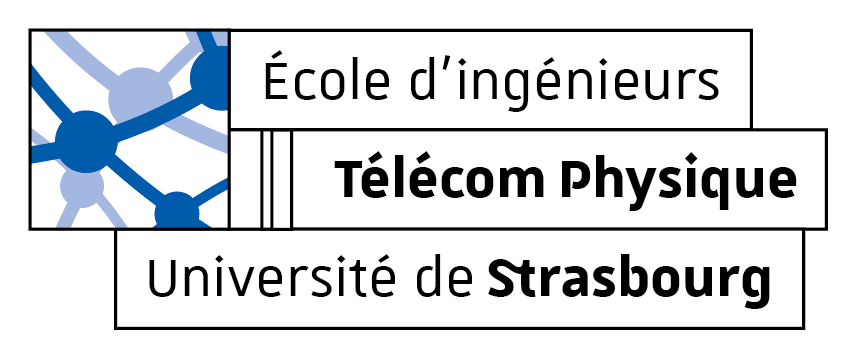
\includegraphics[width=0.35\textwidth]{../tps}\hspace{2 in}
    % \includegraphics[width=0.15\textwidth]{logo_TPS}\hspace{0.2in}
    
\includegraphics[width=0.3\textwidth]{../imt}
    
    \vspace{1cm}
    {\huge
   {\fontfamily{lmss}\selectfont \textbf{Rapport de stage}}\vspace*{0.2cm}
	}
 
    \Huge
    {\fontfamily{lmss}\selectfont\textbf{Evaluation automatique des capacités motrices et d'interaction du bébé pour l'identification précoce des troubles du neurodéveloppement}\vspace*{0.5cm}
       
        {\LARGE  
        \laboratoire}
        \vspace*{0.5cm}
        
        
\includegraphics[width=0.3\textwidth]{../isir}

		{\Large   
			{\periode}\vspace*{0.1cm}
   
			{\etudiant}\vspace*{0.1cm}
   
            {\encadrant}\vspace*{0.1cm}
            
            {\parcours}\vspace*{0.1cm}
            
            {\annee}\vspace*{0.1cm}
		}
    }
    
    	\vspace{0.1in}

    \vfill
         
    
    
    \end{center}
\end{titlepage}


\newpage
\pagestyle{empty}
\clearpage

\Large \textbf{Abstract}
\par 
As part of my first year of a Master's degree in Automatic Signal Processing and Computer Science at Télécom Physique Strasbourg, I did a 4-month placement at the Institut des Systèmes Intelligents et de la Robotique, in the PIROS team, under the supervision of Louis Simon, a PhD student, and Professor Mohamed Chetouani. The aim of this internship was to automatically assess a baby's motor and interaction skills for the early identification of Neurodevelopmental Disorders (NDDs), a group of pathologies affecting the ability to communicate, learn or socialise. One of the major challenges in the treatment of NDDs is early identification and intervention. As part of the TECH-TOYS project, I worked on the application of Bayesian recursive filters, in particular the Kalman filter, for the extraction of descriptor markers for TNDs. The aim was to estimate these motor markers and to assess the robustness of the Kalman filter estimate on the CareToy dataset. Wrist orientation was estimated using an extended Kalman filter, which then allowed us to extract various markers such as \textit{travel path}, \textit{work area}, \textit{work volume} and \textit{jerk}. In assessing the robustness of these descriptors, we found that \textit{travel path} and \textit{work area} were less sensitive to estimation noise.

\Large \textbf{Résumé}
\par
Dans le cadre de ma première année de Master en Automatique Signal et Informatique à Télécom Physique Strasbourg, j'ai effectué un stage de 4 mois à l'Institut des Systèmes Intelligents et de la Robotique, au sein de l'équipe PIROS, sous la supervision de Louis Simon, doctorant, et du Professeur Mohamed Chetouani. Ce stage avait pour objectif l'évaluation automatique des capacités motrices et d'interaction du bébé pour l'identification précoce des Troubles du Neuro-Développement (TNDs), un ensemble de pathologies affectant les capacités à communiquer, apprendre ou encore à socialiser. L'un des défis majeurs dans le contexte de la prise en charge des TNDs est l'identification et l'intervention précoces. Dans le cadre du projet TECH-TOYS, j'ai travaillé sur l'application des filtres récursifs bayésiens, en particulier le filtre de Kalman, pour l'extraction des marqueurs descripteurs des TNDs. L'objectif était d'estimer ces marqueurs de motricité et d'évaluer la robustesse de l'estimation du filtre de Kalman sur le jeu de données CareToy. L'estimation de l'orientation du poignet a été réalisée avec un filtre de Kalman étendu, ce qui nous a ensuite permis d'extraire différents marqueurs tels que le \textit{travel path}, la \textit{surface de travail}, le \textit{volume de travail} et le \textit{jerk}. L'évaluation de la robustesse de ces descripteurs nous a permis de constater que le \textit{travel path} et la \textit{surface de travail} étaient moins sensibles aux bruits d'estimations.
\newpage
\pagestyle{empty}
\clearpage
\Large \textbf{Remerciement}
\par
Je tiens à exprimer ma sincère gratitude envers Mohamed Chetouani pour m'avoir offert l'opportunité enrichissante d'effectuer mon stage au sein de l'équipe PIROS. Je souhaite également adresser mes remerciements les plus chaleureux à Louis Simon pour son encadrement attentif, ses précieux conseils et sa patience inestimable tout au long de cette expérience.
 
\newpage
\pagestyle{empty}
\tableofcontents

\newpage
\pagestyle{empty}
\listoffigures

\newpage
\pagestyle{empty}
\clearpage
\Large \textbf{Présentation ISIR}

L'ISIR (Institut des Systèmes Intelligents et de Robotique) est un laboratoire de recherche affilié à Sorbonne Université, au CNRS et à l'Inserm. Il est situé sur le campus de la faculté des Sciences et d'Ingénierie, place Jussieu à Paris. Le laboratoire regroupe 63 permanents et plus de 121 doctorants travaillant sur la modélisation, le design et les applications de la robotique dans divers domaines, tels que la santé, le transport, les services, l'industrie, etc.

Le laboratoire est divisé en plusieurs équipes :

\begin{enumerate}
    \item L'équipe AGATHE (Assistance aux Gestes et Applications THErapeutiques) : recherche en robotique médicale, notamment les robots d'assistance en chirurgie, les prothèses et le contrôle moteur.
    \item L'équipe AMAC (Architectures et Modèles pour l'Adaptation et la Cognition) : développement de modèles de perception et de cognition inspirés de l'Homme et du Vivant pour améliorer les capacités d'apprentissage et de prise de décision des systèmes robotiques.
    \item L'équipe Interactions Multi-Échelles : travaux sur des interfaces matérielles et logicielles adaptées à l'humain, sur plusieurs échelles spatiales et temporelles.
    \item L'équipe MLIA (Machine Learning \& deep learning for Information Access) : recherches sur l'apprentissage machine et ses applications.
    \item L'équipe PIROS (Perception, Interaction et Robotique Sociale) : concentration sur la compréhension, la mesure et l'utilisation des signaux sociaux dans les interactions humain-humain ou humain-robot. Cette équipe regroupe des spécialistes en robotique, traitement du signal, apprentissage machine, psychologie et sciences cognitives.
    \item L'équipe SYROCO (SYstèmes RObotiques COmplexes) : travaille sur la conception et le contrôle de systèmes robotiques complexes.
\end{enumerate}

Par ailleurs, l'ISIR est à l'origine de nombreuses start-up et contribue au transfert de technologies vers l'industrie à travers une structure interne labellisée : l'Institut Carnot.

\newpage
\pagestyle{fancy}
\setcounter{page}{1}
\section{Introduction}
Les troubles du neuro-développement (TNDs) représentent un défi majeur de santé publique, affectant la croissance et le développement du cerveau chez les nourrissons et les jeunes enfants. Ces altérations peuvent engendrer une diversité de déficiences fonctionnelles, comprenant des troubles cognitifs, moteurs, du langage, de l'apprentissage et du comportement, souvent résultant de diverses causes, qu'elles soient génétiques, lésionnelles ou environnementales \cite{development_americas_nodate}.

La détection précoce des nourrissons présentant un risque de TNDs revêt une importance capitale pour la mise en place de programmes d'intervention efficaces. Cependant, les méthodes cliniques traditionnelles de détection peuvent être sujettes à des limitations, notamment en termes de subjectivité, de temps requis et d'accessibilité. L'évaluation clinique, bien que cruciale, peut être fastidieuse et peu adaptée à une observation écologique dans des contextes naturels de la vie quotidienne.

Face à ces défis, les avancées en ingénierie neuro-développementale (IND) et l'utilisation des technologies informatiques ouvrent de nouvelles perspectives. Le projet TECH-TOYS s'inscrit dans cette démarche en proposant de nouvelles méthodes et outils pour comprendre les mécanismes neuro-biologiques du développement du cerveau humain, analyser quantitativement le comportement humain pendant le développement neurologique et évaluer les étapes de ce développement dès la naissance.

Ce rapport se concentre sur l'extraction des descripteurs moteurs à partir des méthodes de traitement du signal, en mettant particulièrement l'accent sur l'utilisation du filtre de Kalman. Nous évaluons la robustesse de cette extraction de descripteurs face aux différentes incertitudes liées à l'estimation des filtres, ainsi qu'aux différentes hypothèses prises en compte, en utilisant un dataset de diverses trajectoires émulées. Après avoir introduit le projet TECH-TOYS ainsi que le concept d'ingénierie neurodéveloppementale dans la section \ref{contexte}, nous discuterons des principaux éléments théoriques ainsi que des modèles de filtre utilisés pour l'estimation de trajectoire dans la section \ref{modèle}. Le protocole expérimental mis en œuvre ainsi que les résultats seront ensuite présentés en détail dans la section \ref{expé}. Enfin, les limites seront exposées dans la section \ref{limites}.
\newpage
\section{Contexte}
\label{contexte}
\subsection{Approche clinique et ingénierie neuro-développementale}
\par Les \textit{troubles du  neuro-développement} (TNDs) sont des altérations de la croissance et du développement du cerveau qui affectent plusieurs fonctions cérébrales, et comprennent les troubles cognitifs, moteurs, du langage, de l'apprentissage et du comportement dus à de nombreuses causes  génétiques, lésionnelles et environnementales.\cite{development_americas_nodate}. Les nourrissons (jeune bébé de la naissance à 12 mois)  présentant un risque élevé sont ceux nés prématurément (\textit{i.e.} nés à moins de 37 semaines d'âge gestationnel)\cite{cecchi_caretoy_2016}, selon l'organisation mondiale de la santé ces derniers représenteraient chaque année 15 millions de naissances dans le monde et seraient en croissance en raison de l'augmentation du taux de survie\cite{blencowe_national_2012}.\\
La \textit{détection précoce} (\textit{i.e.} au cours des premières semaines ou mois de vie) des nourrissons présentant un risque de TNDs grâce à une évaluation clinique minutieuse (\textit{i.e.} des tests de développement, un examen neurologique, observation des mouvements spontanés) combinée à des des outils techniques spécifiques tels que la neuro-imagerie (ultra-sons crâniens, imagerie par résonance magnétique du cerveau [IRM]), des tests neurophysiologiques (\textit{e.g.} électroencéphalographie) et les tests génétiques (caryotype, hybridation génomique comparative - microréseau)\cite{cioni_early_2016}  est une condition préalable majeure pour les programmes d'intervention et joue un rôle important dans l'efficacité de la rééducation\cite{orton_early_2009,spittle_early_2015}. Cependant les méthodes cliniques de détection des TNDs requièrent souvent un apport subjectif de la part de professionnels qualifiés, prennent du temps et peuvent être fastidieuses à évaluer. Les sessions d'évaluation regroupent généralement plusieurs examens à la suite. La réalisation de cette évaluation peut être fatigante pour l'enfant. En outre, ces évaluations ne permettent pas de réaliser des examens écologiques (\textit {in situ}), dans le contexte de la vie quotidienne.  Par conséquent, ces tests sont peu accessibles et les listes d'attente de six mois ou plus sont fréquentes, même dans les pays les plus riches \cite{gargot_automatic_2022}.\\

\par Les technologies informatiques offrent la possibilité de surmonter ces obstacles, de caractériser le comportement des enfants dans des contextes plus naturels. Ce défi a été relevé par l'ingénierie neuro-développementale (IND)
\cite{campolo_novel_2008,campolo_neuro-developmental_2010} dans le but de fournir de « nouvelles méthodes et de nouveaux outils » pour: (1) Comprendre les mécanismes neuro-biologiques du développement du cerveau humain; (2) Effectuer une analyse quantitative et une modélisation du comportement humain pendant le développement neurologique; (3) Évaluer les étapes du développement neurologique atteint par les humains à partir de la naissance \cite{campolo_neuro-developmental_2010}.
Les applications sont nombreuses et comprennent la robotique \cite{scassellati_improving_2018,jouaiti_robot-based_2019}, les jeux informatiques \cite{grossard_serious_2017}, le diagnostic \cite{bangerter_autism_2017,hashemi_computer_2014} et l'imagerie comportementale \cite{torres_characterization_2016,anzalone_how_2014,anzalone_quantifying_2019}. Le Machine Learning (ML), le Deep Learning (DL) \cite{zemouri_deep_2019,mahmud_deep_2021} en particulier, est de plus en plus utilisé en médecine \cite{triantafyllidis_applications_2019,mahmud_deep_2021} en particulier en psychiatrie \cite{koppe_deep_2021}.

\subsection{Le projet TECH-TOYS}
\subsubsection{Le projet CareToys}
\par Le projet CareToys \cite{noauthor_project_nodate}, \cite{cecchi_caretoy_2016} est un projet clinique d’intervention clinique mené entre 2013 et 2016 par IRCCS Fondazione Stella Maris et un ensemble de collaborateurs européens. Cette initiative, qui préfigure le projet TECH-TOYS, est centrée autour d’un dispositif intelligent, sous la forme d’un environnement de jeu pour bébé, permettant la conduite de programmes d’intervention précoce personnalisés, intensifs, à la maison et centrés sur la famille. Un ensemble d’algorithmes ont été utilisés afin d’analyser le mouvement de l’enfant \cite{rihar_infant_2014} ainsi que ses capacités de saisie \cite{del_maestro_sensing_2011}. Un essai clinique \cite{sgandurra_home-based_2014} a été mené afin de tester le système sur des enfants de 3 à 9 moins nés avant terme et à risque de développer une paralysie cérébrale, un trouble affectant les capacités motrices tout au long de la vie. Cet essai clinique avait aussi pour but de tester les hypothèses suivantes : \begin{itemize}
    \item L’utilisation d’un système intelligent permet d’améliorer le développement moteur, perceptuel et cognitif du bébé
    \item Le dispositif modulaire développé permet d’assister les soignants dans le processus d’intervention précoce
    \item Le système de télé-réhabilitation développé représente une nouvelle forme crédible de prise en charge des troubles du neuro-développement
\end{itemize} 
En parallèle de l’utilisation du dispositif de réhabilitation, un ensemble de tests ont été menés par les équipes cliniques afin d’évaluer l’efficacité du système, e.g l’Infant Motor Profile \cite{heineman_infant_2008}.\\
Ce projet a permis de mettre en lumière les bénéfices de l’intervention précoce à la maison à l’aide d’un dispositif intelligent. Un effet positif et significatif sur les capacités motrices de l’enfant après quatre mois d’intervention a été observé après comparaison du score IMP des bébés ayant suivis un programme de réhabilitation avec le dispositif CareToys et ceux ayant suivis un soin classique \cite{sgandurra_effects_2019}.

\subsubsection{Origine et résumé du projet}
\par Le projet TECH-TOYS est issu de l’appel à projet d’ERA PerMed portant sur la recherche multidisciplinaire
en médecine personnalisée, financé en France par l’Agence Nationale de la Recherche. Il regroupe un ensemble de collaborateurs académiques et privés en Europe ayant des expertises en psychiatrie, robotique/intelligence artificielle, ingénierie et droit. L’objectif de ce consortium est de développer une technologie permettant la détection précoce des troubles du neurodéveloppement chez le bébé à domicile de façon quantitative.\\
La session 2021 d’EraPer Med, dont le projet TECH-TOYS émane, avait pour sujet le développement
d’outils de soutien clinique pour la mise en oeuvre de la médecine personnalisée. Cet appel à projet avait
pour but de sélectionner des projets de recherche européens « interdisciplinaires et démontrant clairement l’impact potentiel de la médecine personnalisée ainsi que la valeur ajoutée par la collaboration transnationale »\cite{noauthor_joint_nodate}. Afin d’être sélectionné, chaque projet devait couvrir les trois modules suivants : 1) La recherche clinique, 2) L’application dans le domaine de la santé, caractérisé par une utilisation des technologies de l’information et de la communication (TIC), et 3) La prise en compte des aspects éthiques, légaux et sociétaux (ELSA). Ci-dessous les contributions majeures, par modules, amenées par le projet
TECH-TOYS :
\begin{table}[H]
\begin{tabularx}{\textwidth}{|p{0.25\textwidth}|X|}
\rowcolor{lightgray}
Module & Apport du projet TECH-TOYS\\
\hline
Recherche clinique &  
                        \begin{itemize}
                        \item L’utilisation combinée de biomarqueurs cliniques et numériques pour la création d’un \textit{phénotype numérique} permettant la détection et le suivi précoce du développement du bébé.
                        \item Un algorithme de Machine Learning pour la stratification et l’identification de phénotypes spécifiques.
                        \item Le déploiement d’outils de télémedecine à domicile durant l’étude clinique.
                      \end{itemize}
                     \\
\hline

Application à l'aide des TIC &  \begin{itemize}
                        \item L’utilisation de données antérieures et nouvellement acquises pour l’entraînement de modèles d’apprentissage non-supervisés et explicables permettant de mieux comprendre le lien entre la présence ou l’absence des différents biomarqueurs.
                        \item Un outil de diagnostic pour les bébés à risque permettant de formaliser rapidement l’information fournie par les modèles de ML précédemment décrits.
                      \end{itemize}
                     \\
\hline
Prise en compte ELSA & \begin{itemize}
                        \item Un système customisable et adapté à tous les enfants et familles, quel que soit le statut socio-économique.
                        \item Un système respectant le règlement général sur la protection des données.
                      \end{itemize}\\
\hline

\end{tabularx}
\caption{Contributions du projet TECH-TOYS}
\label{}
\end{table}
\par Ce projet regroupe les cinq partenaires suivants : IRCCS Fondazione Stella Maris (FSM) représentée par Professeur Giovanni Cioni, le département de psychiatrie de l’enfant et de l’adolescent de la Pitié Salpêtrière (APHP) représenté par Professeur David Cohen, l’Institut des Systèmes Intelligents et de Robotique (ISIR) représenté par Professeur Mohamed Chetouani, l’université Ludwig Maximilians (LMU) représentée par PD. Dr. Fiorella Battaglia, la startup Khymeia S.r.l. (KHY) représentée par Marco Pirini,
PhD, et l’université Technologique d’Istanbul (ITU) représentée par Professeure Hatice Kose.\\
Le projet TECH-TOYS, acronyme de \textit{acquire digiTal biomarkErs in infanCy witH sensorized TOYS for
early detection and monitoring of neurodevelopmental disorders}, a pour objectif d’améliorer la détection
précoce des TNDs chez le bébé en combinant l’étude des comportements moteurs et l’étude de l’interaction
enfant-soignants. Le projet de recherche se focalisera en particulier sur les bébés prématurés ou nés à terme
avec des lésions cérébrales congénitales et ayant de forts risques de développer une paralysie cérébrale ou
autres formes modérées de TNDs. Pour se faire, un environnement de jeu ainsi qu’un ensemble d’algorithmes
et modèles d’apprentissage machine vont être développés afin d’assister les professionnels de santé dans
la détection et le suivi des bébés à risque. Le projet, d’une durée de 36 mois, se déroulera en plusieurs
phases : 1) L’analyse de données et le design du baby-gym 2) Le test et l’évaluation des modèles d’analyse
de données durant l’essai clinique prospectif 3) Le déploiement du baby-gym à domicile et la validation des
modèles. La partie analyse de données sera basée en partie sur l’utilisation des données issues du projet
CareToys \cite{rihar_infant_2019}, un projet mené par les équipes de FSM. Mené entre 2011 et 2015, ce projet
a conduit au développement d’un système modulaire pour l’intervention précoce personnalisée et adaptée à l’environnement familial permettant la stimulation et le suivi d’enfants prématurés à risque de développer une paralysie cérébrale.

\subsubsection{Modules d'ingénierie}
\par Le travail des ingénieurs et chercheurs en robotique et IA sera partagé entre trois des modules du projet : a) Le design du dispositif de jeu TECH-TOYS, b) l’analyse de données, avec le développement d’un modèle de phénotypage et c) Le modèle de médecine de précision.\\ \\
 
\textbf{Le baby-gym TECH-TOYS :} Les données nécessaires seront acquises via un système de baby-gym
composé d’un matelas sensorisé, de centrales inertielles (IMUs) placées sur l’enfant et le soignant ainsi que d’un ensemble de caméras et micros (voir figure \ref{fig:gym}). Le dispositif developpé sera similaire à celui utilisé pour le projet CareToys , à l’exception d’une caméra supplémentaire qui filmera à la fois l’enfant et le parent pour étudier leurs interactions ainsi que des micros pour analyser les vocalisations du bébés et le mamanais, i.e. le discours, caractérisé entre autre par une prosodie inhabituelle, employé par les parents pour communiquer avec bébé.
\begin{figure}[H]
    \begin{subfigure}{1\textwidth}
        \centering
        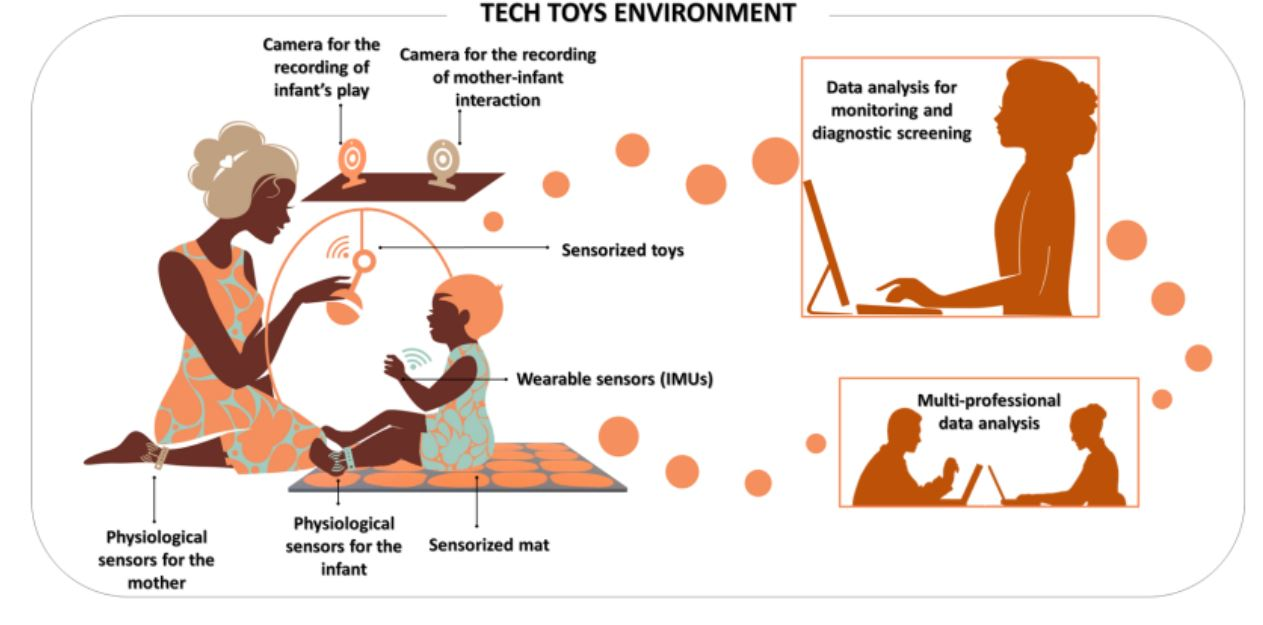
\includegraphics[width=\linewidth, height=8cm]{../TT env.jpg}
        \caption{Environnement TECH-TOYS}
        \label{subfig:gyma}
    \end{subfigure}
    \begin{subfigure}{1\textwidth}
    \centering
        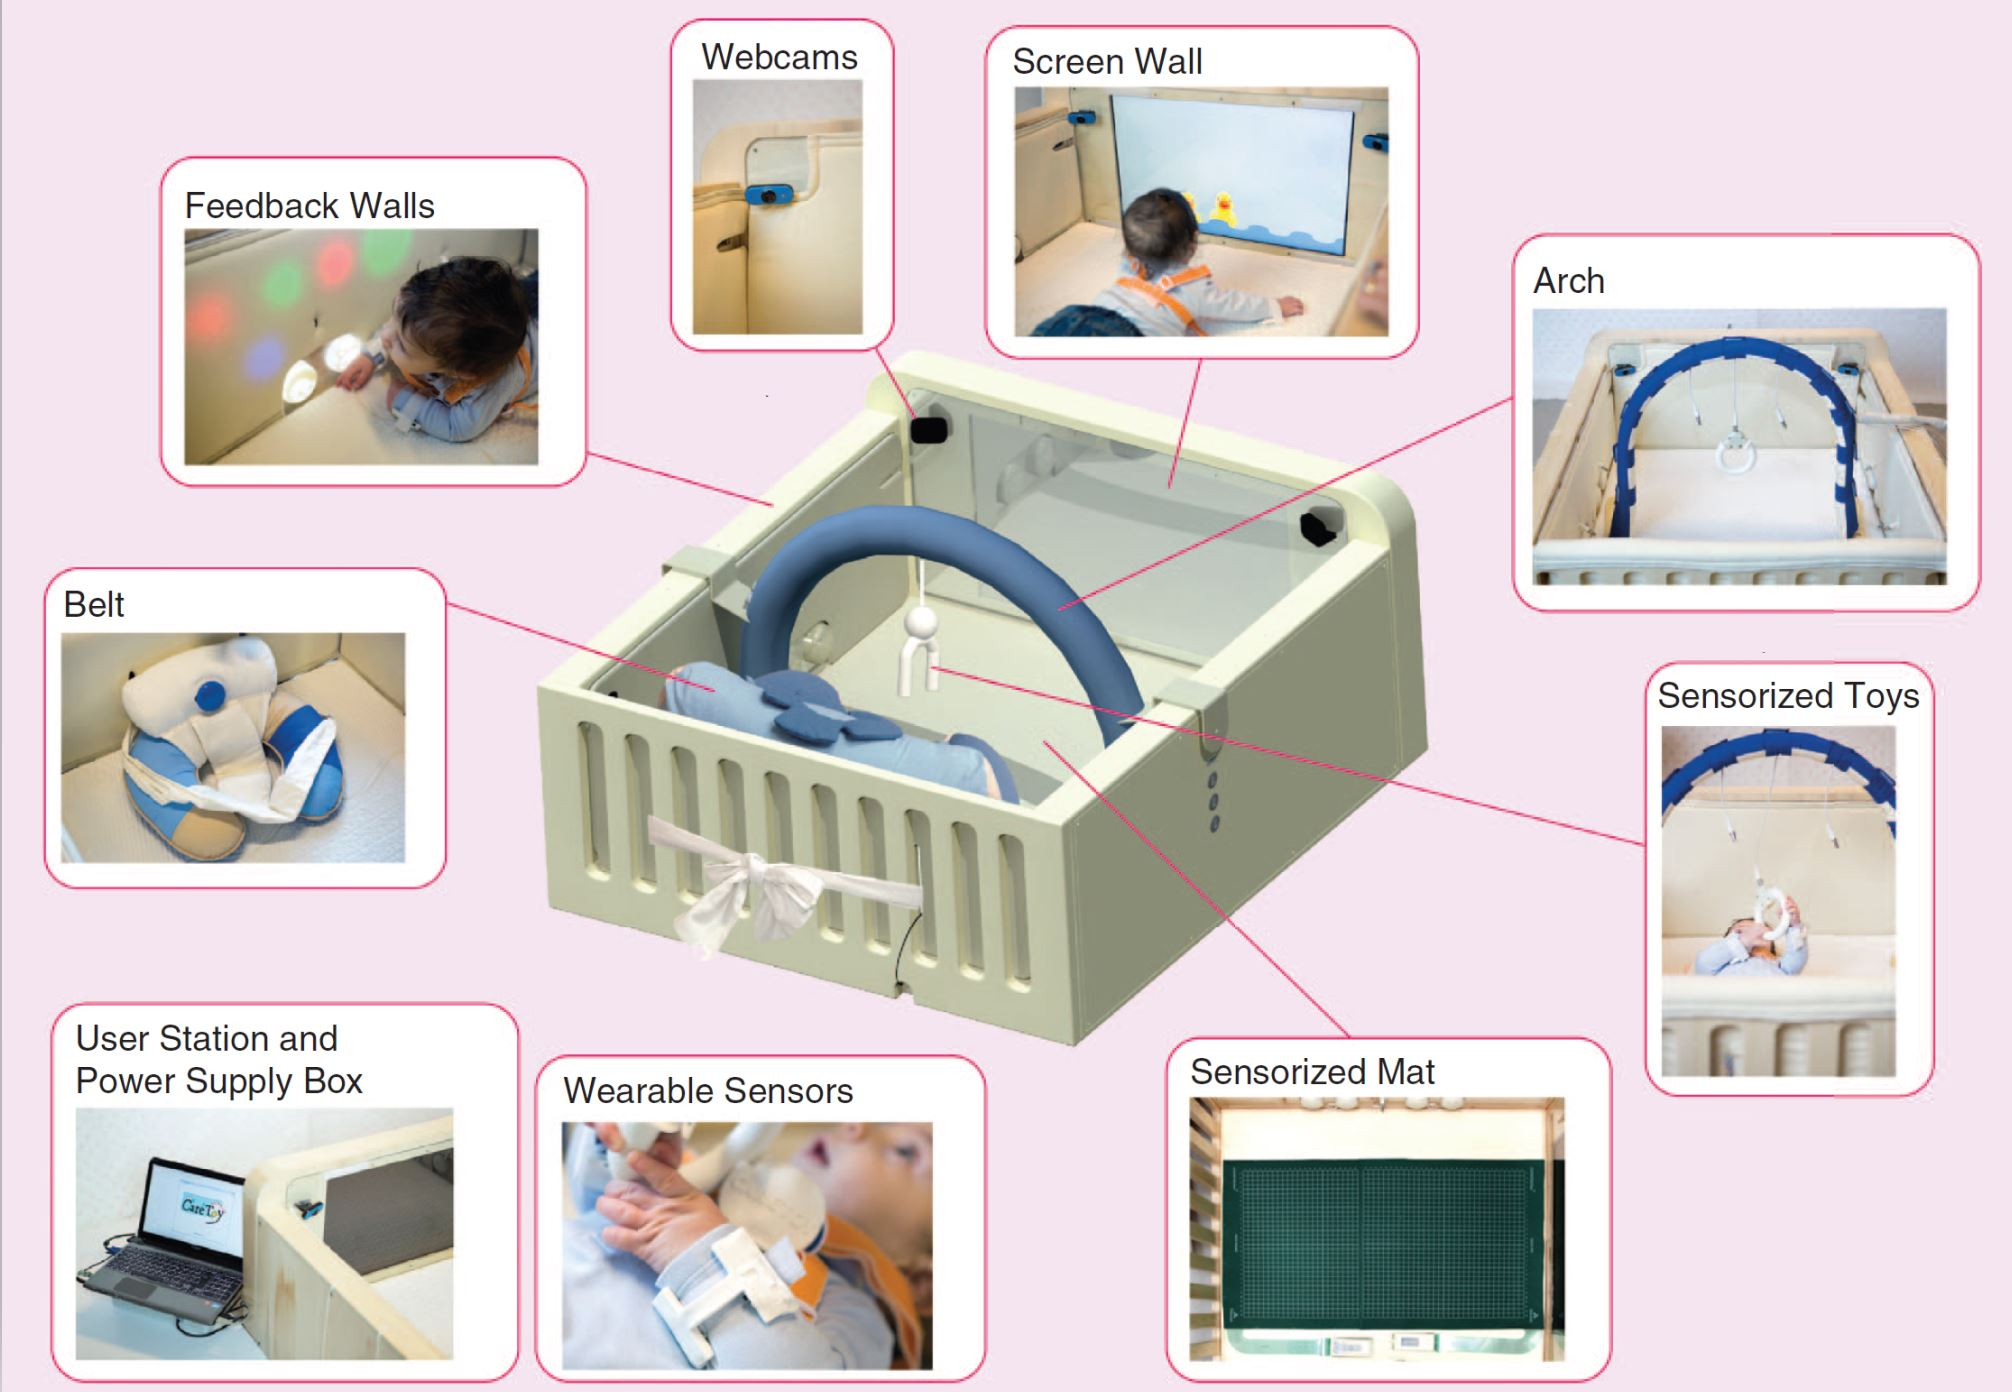
\includegraphics{../babygym.jpg}
        \caption{Dispositif CareToys, source : \cite{cecchi_caretoy_2016}}
        \label{subfig:gymb}
    \end{subfigure}
    \caption{Dispositif de détection et d’intervention précoce TECH-TOYS}
    \label{fig:gym}
    \footnotesize
    \vspace{.2cm}
    Une fois déployé à la maison, le dispositif TECH-TOYS permettra d’acquérir des données physiologiques du bébé et d’un des parents via les IMUs, d’étudier la posture et le mouvement du bébé à l’aide du tapis de pression ainsi que l’interaction
à l’aide des caméras. Les données ainsi récoltées pourront être directement analysées par les cliniciens et les modèles de ML grâce à une communication avec un serveur sécurisé (figure \ref{subfig:gyma}). Le dispositif développé s’inspirera en grande partie de celui mis en place durant le projet CareToys (figure \ref{subfig:gymb}) qui a déjà permis de récolter des données pertinentes pour l’intervention précoce.
\end{figure}
\vspace{2cm}
\textbf{L'analyse de données : } La première partie du projet consistera à sélectionner, sur la base de données précédemment acquises, un ensemble d’indicateurs cliniques et computationnels permettant d’évaluer les capacités motrices et d’interactions des bébés. En particulier, l’activité des membres supérieurs, de la posture ainsi que de l’interaction parents-enfant seront analysés en détails. Ci-dessous une liste exhaustive des comportements qui pourront être étudiés :
 \begin{itemize}
     \item Comportements moteurs : Saisie d’objets, mouvement des membres supérieurs, mouvement pour
atteindre des objets, manipulation, posture, dynamique du corps
\item Comportements liés à l’interaction : Synchronie, vocalisation, dynamique des interactions vocales
(e.g le turn taking), attention conjointe
 \end{itemize}
 Les séquences de comportements ainsi extraites permettront d’identifier des biomarqueurs numériques de
la paralysie cérébrale (CP) ou d’autres TNDs. On appelle biomarqueur l’indicateur, ici numérique, de la
présence ou l’absence d’un trouble. Ces biomarqueurs permettront de définir un phénotype pour chaque
diagnostic, e.g, un dictionnaire regroupant tout les comportements liés à une condition (CP, TNDs, ou
typique) ainsi que leur niveau d’expressivité. Ces phénotypes permettront à termes aux professionnels de
santé d’obtenir une évaluation quantitative des capacités motrices et d’interactions du bébé afin de mieux
planifier de futures interventions ou aider à l’établissement du diagnostic. \\
\textbf{Le modèle de médecine de précision : } La médecine de précision désigne le processus de définition
d’une pathologie au moyen de techniques génomiques ou encore computationnelles, permettant un ciblage
plus précis des différentes formes de ladite pathologie. Dans le cadre du projet TECH-TOYS, un
outil de médecine de précision sera mis en place afin d’assister les cliniciens dans l’observation et la prise
de décisions au regard du diagnostic et de l’intervention. \\

La dernière partie, qui n'est pas pertinente pour le cadre de mon stage, ne sera pas abordée dans la suite du rapport.

\subsubsection{Objectifs du stage}

Le stage a pour objectif de contribuer à la compréhension et à l'analyse du développement moteur chez les enfants à risque de troubles neurodéveloppementaux. Les données d'IMUs (Inertial Measurement Units) collectées grâce au baby-gym sont un outil précieux pour collecter des informations sur les mouvements corporels et la coordination motrice. Dans ce contexte, nous chercherons à extraire des descripteurs de finesse tels que le "jerk" (variation de l'accélération) et le "travel path" (chemin parcouru), la surface et le volume de travail à partir de ces données, ce qui permettra d'obtenir des informations détaillées sur les mouvements des enfants. \\
\textbf{Acquisition de données IMU :} Il s'agit d'apprendre la mise en œuvre et la configuration des IMUs (Unités de Mesure Inertielle) pour la collecte de données relatives aux mouvements corporels des enfants. Cela implique de comprendre le placement adéquat des capteurs et la réalisation de la calibration. À cet effet, un protocole expérimental ainsi que des spécifications techniques (caractéristiques requises des IMUs, méthodes de placement et de calibration) ont été élaborés pour remédier aux lacunes identifiées dans le dispositif Baby-Gym CareToys, dans le cadre du projet Tech Toys.\\
\textbf{Extraction des caractéristiques de finesse :} Cette étape consiste à développer des algorithmes et des scripts de traitement du signal (en utilisant, par exemple, le filtre de Kalman) en vue d'extraire des paramètres tels que le jerk (variation de l'accélération) et la trajectoire de déplacement à partir des données IMU. Ces paramètres permettront d'obtenir des informations sur la fluidité des mouvements ainsi que sur la précision des gestes effectués.\\
\textbf{Analyse statistique :} Dans cette phase, des méthodes statistiques sont employées pour analyser les paramètres extraits. Cette analyse comprend l'évaluation de la robustesse des paramètres face aux variations et à l'incertitude des paramètres d'estimation, ainsi que la capacité des algorithmes d'estimation à généraliser leur performance sur diverses trajectoires.

Ce stage vise à combiner la technologie des IMUs avec l'analyse des données pour mieux comprendre le développement moteur chez les enfants à risque de troubles neurodéveloppementaux. L'extraction de descripteurs de finesse à partir de ces données contribuera à une évaluation plus précise des performances motrices et pourrait avoir des implications importantes dans le diagnostic précoce et la prise en charge des enfants concernés.
% Détailler les objectifs en les liant avec le contexte et les modules d'ingénierie précedemment présentés.


\newpage
\section{État de l'art}
\subsection{Évaluation clinique des comportements moteurs}
\label{subsec: assess_sensor}

\par L'évaluation des comportements moteurs chez les nourrissons revêt une importance particulière avant leur premier anniversaire, car c'est à cette période que les bases de leurs capacités motrices futures sont établies \cite{adolph_physical_2005}.  Les évaluations neuromotrices précoces peuvent s'avérer complexes, car le développement moteur au cours de la première année de vie est à la fois rapide et étendu, et il est influencé par une combinaison de facteurs biologiques, environnementaux et sociaux. Les \textit{méthodes cliniques} couramment utilisées, telles que l'AIMS (Alberta Infant Motor Scale), le TIMP (Test of Infant Motor Performance) et le Bayley III [51], exigent une expertise approfondie ainsi qu'un œil exercé de la part des cliniciens pour être correctement appliquées.\\

\textbf{L'Alberta Infant Motor Scale (AIMS)} est un outil normalisé qui a été développé pour évaluer le développement de la motricité globale chez les nourrissons, de la naissance (40 semaines de conception) jusqu'à l'âge de marche autonome (18mois) \cite{noauthor_motor_nodate}. Cette échelle a été créée dans les années 1990 par Martha C. Piper et Johanna Darrah de l'Université de l'Alberta, au Canada\cite{noauthor_motor_nodate},et elle se compose d'une feuille de résultats ainsi que d'un manuel d'instructions \cite{noauthor_motor_nodate}. La feuille de score de l'AIMS comprend un total de 58 items, répartis en quatre positions (21 en position couchée, 9 en position ventrale, 12 en position assise et 16 en position debout).Chaque item évalue les composantes du développement moteur en se basant sur trois éléments principaux : le port de poids, la posture et les mouvements antigravitaires. Cette échelle prend en considération à la fois les aspects quantitatifs et qualitatifs du développement moteur, en couvrant des étapes importantes telles que le pivotement, la roulade, la reptation réciproque, la position assise et la marche. L'un des avantages majeurs de l'AIMS est sa simplicité et sa rapidité d'administration, en plus de sa relative facilité d'utilisation \cite{eliks_alberta_2022}. Cependant, il convient de noter que la version originale de l'AIMS a été développée au Canada, et les scores normatifs qu'elle fournit sont basés sur une population canadienne de nourrissons. Par conséquent, son utilisation dans d'autres contextes culturels nécessite une adaptation et une validation spécifique. Ce processus d'adaptation comprend la traduction de l'outil dans une nouvelle langue, la synthèse des traductions, la rétrotraduction sémantique, idiomatique, expérimentale et conceptuelle, ainsi que le test de la version préliminaire et la mesure de sa fiabilité et validité \cite{boateng_best_2018}. De plus, il est important de noter que la fiabilité interévaluateur (la cohérence des résultats entre différents évaluateurs) et la fiabilité intra-évaluateur (la cohérence des résultats lorsqu'un même évaluateur répète la mesure dans des conditions identiques) ne sont pas toujours garanties, ce qui peut présenter des limites dans son utilisation clinique. Ces lacunes ont conduit à l'exploration de méthodes d'automatisation des évaluations cliniques, en utilisant les technologies de l'information et de la communication (TIC), dans le but d'améliorer la précision, la reproductibilité et la fiabilité de ce processus dans différents contextes.\\
 
Plusieurs travaux ont joué un rôle essentiel dans l'avancement des méthodes d'évaluation des comportements moteurs des nourrissons en utilisant une variété de technologies, notamment des systèmes d'acquisition d'images optiques, des capteurs de pression, des centrales magnétiques et inertielles, entre autres. Ci-dessous, voici une liste de différentes outils/méthodes d'évaluation des comportements moteurs du nourrisson, accompagnée de leur description, de leurs avantages et de leurs limites :
\begin{itemize}
    \item \textbf{Caméras numériques}
    \begin{itemize}[label={\textbullet}, leftmargin=*]
        \item Description et Apport :  Elles ont  été utilisées avec un codage et une classification supplémentaire de bandes vidéos pour étudier l'influence du contrôle postural sur le comportement de la main\cite{rocha_influence_2008} et le comportement de préhension du nourrisson par rapport à la préférence pour la main \cite{marschik_reaching_2008}. 
        \item Limites :  Souffrent d'obstruction, nécessitent un calibrage complexe de la caméra, l'éclairage des marqueurs et des réglages minutieux du zoom et de la mise au point.
    \end{itemize}
    \item \textbf{Systèmes optoélectroniques multi-caméras}
    \begin{itemize}[label={\textbullet}, leftmargin=*]
        \item Description et Apport : (Optotrak, Vicon, Qualisys motion capture) exploitent les avantages du spectre infrarouge et garantissent une précision inférieure à 1 mm, même à des fréquences d'échantillonnage élevées \cite{petitto_baby_2004}.
        \item Limites :  Le nombre élevé de marqueurs nécessaires, le système est invasif, la préparation fastidieuse du sujet et du système de mesure. Bien que la complexité peut être réduite grâce aux groupes de marqueurs, de grands segments de données manquantes dues aux mouvements inattendus du nourrisson et de l'auto-occlusion restent un problème.
    \end{itemize}
    \item \textbf{Électromyographie (EMG)}
    \begin{itemize}[label={\textbullet}, leftmargin=*]
        \item Description et Apport : Utilisée en complément avec un système basé sur une caméra optique pour extraire les meilleures informations sur le mouvement et les données d'activation musculaire, afin d'étudier le contrôle postural pendant les taches de préhension du nourrisson \cite{van_der_fits_postural_1999,de_graaf-peters_postural_2007}.
        \item Limites : Système invasif et requiert des méthodes de détection,
        décomposition, de traitement et de classification avancées \cite{raez_techniques_2006}.
    \end{itemize}
    \item \textbf{Systèmes de suivi électromagnétique}
    \begin{itemize}[label={\textbullet}, leftmargin=*]
        \item Description et Apport : Ils ont été utilisés en coopération avec les méthodes d'élimination et de déplacement des capteurs de mouvement \cite{karch_quantification_2008} pour dépasser les exigences en matière de visibilité directe des systèmes optiques \cite{karch_compensation_2010}.
        \item Limites : Souffrent de limitation de mouvement due au câblage.
    \end{itemize}
    \item \textbf{Accéléromètres}
    \begin{itemize}[label={\textbullet}, leftmargin=*]
        \item Description et Apport :  Ils ont été utilisés pour l'analyse des mouvements spontanés \cite{ohgi_time_2008} des extrémités supérieures \cite{gima_dynamical_2011} et inférieures du nourrisson, mais ne fournissent pas d'informations sur la posture.
        \item Limites : Sensibles aux bruits de mesure et pas adaptés pour les mouvements à grande variation angulaire.
    \end{itemize}
    \item \textbf{Centrales inertielles et magnétiques sans fil}
    \begin{itemize}[label={\textbullet}, leftmargin=*]
        \item Description et Apport : Ce sont des systèmes portables, non invasifs
            et peu coûteux composés d’un gyroscope à trois axes, d’un accéléromètre à trois axes
            et d’un magnétomètre à trois axes. Cet ensemble de capteur mesurent la vitesse angulaire tridimensionnelle, l’accélération et le vecteur champs magnétique.
        \item Limites : Sensibles aux bruits de mesure
    \end{itemize}
    \item \textbf{Matélas à répartition de pression}
    \begin{itemize}[label={\textbullet}, leftmargin=*]
        \item Description et apport : Ce sont des matrices de capteurs à effet piezorésistifs. Les applications existantes sont plus nombreuses dans le domaine de l’analyse de la posture des adultes , comme l’analyse non invasive des habitudes de sommeil \cite{ni_towards_2010,metsis_non-invasive_2014} et les méthodes de prévention des ulcères \cite{yousefi_bed_2011}.
        \item Limtes : Limitations de l'échantillonnage, la résolution spatiale des capteurs de pression dans les matelas peut limiter la précision des données, en particulier pour les mouvements fins ou rapides.
    \end{itemize}
\end{itemize}

\subsection{Évaluation de la motricité du bras des enfants à risque de TNDs}

\par L'étude visant à évaluer les comportements moteurs du bras chez les nourrissons a révélé des développements atypiques chez les enfants présentant un risque de troubles neurodéveloppementaux (TNDs). Cette évaluation repose sur l'analyse de diverses mesures cinématiques et des aspects géométriques du mouvement. Elle englobe la description de la position, de la vitesse, de l'accélération/décélération des points de l'objet en mouvement. La combinaison de ces mesures permet d'estimer des caractéristiques telles que la trajectoire, la courbure, le jerk (variation de l'accélération), la fluidité, la rectitude, la complexité et la régularité du mouvement. De plus, cette analyse peut également prendre en compte les interactions du nourrisson avec son environnement, notamment l'espace/volume de travail, la manière dont il saisit et interagit avec les objets qui l'entourent. \\  
L'étude menée par \textcite{ouss_developmental_2018} consiste à extraire les trajectoires des mouvements de la main (MMs) à partir d'enregistrements vidéo impliquant des nourrissons âgés de 2 à 10 mois. Ces nourrissons sont regroupés en différentes cohortes, notamment ceux à risque de troubles neurodéveloppementaux (TNDs) tels que le syndrome de West (SW), les prématurés (P), les enfants présentant des troubles oraux (TO), ceux issus de mères malvoyantes (MV), et ceux ayant subi une hospitalisation précoce (HP). Ces nourrissons sont comparés à des témoins qui interagissent avec leur mère dans un contexte interactif. Ils se posent les questions de recherche suivantes: 1) Les MMs diffèrent-ils avec l'âge dans toutes les cohortes ? 2) Est-ce que les MMs diffèrent en fonction du contexte (interaction avec une personne ou un objet) ? 3) Les MMs diffèrent-ils selon les cohortes: témoins ou à risque de TNDs ? et 4) Peut-on utiliser les MMs comme des indicateurs cliniques des TNDs ? Pour répondre à ces questions, ils ont calculé divers descripteurs de trajectoires basés sur les métriques cinématiques, comprenant des statistiques telles que la moyenne, le minimum, le maximum, l'écart-type, les pauses, etc. Ensuite, ils ont effectué des analyses statistiques, notamment un regroupement hiérarchique basé sur l'indice de corrélation de Pearson pour évaluer la similarité entre les différents descripteurs. Ils ont également utilisé le test non paramétrique d'analyse de variance de Kruskal-Wallis pour évaluer les différences entre les cohortes, suivi d'un test de Dunn pour identifier précisément les groupes ayant des effets différents. Enfin, ils ont testé les interactions entre l'âge et la cohorte à l'aide d'une ANOVA de type III. Les résultats principaux de l'étude sont les suivants : 1) Les caractéristiques cinématiques des MMs étaient significativement liées à l'âge dans toutes les cohortes, 2) Les MMs différaient significativement à l'âge de 5-6 mois chez les nourrissons témoins, selon le contexte 3) Les trajectoires développementales des MMs étaient influencées de manière significative par des facteurs environnementaux et développementaux dans différentes cohortes, avec l'environnement jouant un rôle pour les nourrissons MV, le développement pour les nourrissons P et SW, et les deux facteurs pour les nourrissons TO et 4) Les courbures du MM ont montré un développement atypique chez les nourrissons SW lorsque l'âge de développement était pris en compte. 

\textcite{muty_detecting_2016} ont développé un système visant à détecter de manière automatique les mouvements du bras en se basant sur un score de symétrie du bras. Ce score est calculé en utilisant une modélisation de l'estimation de la posture humaine et la représentation du squelette à partir de vidéos provenant d'une base de données publique comprenant de jeunes enfants qui ont reçu un diagnostic de trouble du spectre autistique. Dans l'étude menée par \textcite{quijano-gonzalez_upper_2014}, un système de suivi de mouvement à l'aide de 6 caméras a été utilisé pour suivre la trajectoire tridimensionnelle du poignet chez des enfants âgés de 6 à 12 ans, qu'ils présentaient un risque de paralysie cérébrale (PC) ou non. Les enfants ont été observés alors qu'ils interagissaient avec des jouets, notamment en remplissant et vidant une boîte de tri contenant divers objets géométriques \cite{klein_instrumented_2011}. Dans le but d'analyser les performances des enfants dans différentes tâches, trois indicateurs de finesse ont été utilisés, à savoir le "jerk" logarithmique sans dimension (JLD), la longueur de l'arc spectral (LAS) et le nombre de pics (NP). Les résultats de l'étude ont révélé que les valeurs JLD, LAS et NP obtenues à partir des côtés affectés des enfants atteints de PC étaient généralement plus élevées que la moyenne observée dans le groupe témoin. En revanche, les côtés non affectés des enfants atteints de PC présentaient des valeurs de ces indicateurs plus faibles que leurs côtés affectés, bien que ces valeurs n'atteignent pas systématiquement celles du groupe témoin. En conséquence, il a été constaté que les enfants souffrant de déficiences motrices éprouvaient des difficultés à contrôler la vitesse de leur membre supérieur affecté, ce qui se reflétait dans les mesures obtenues. L'absence de mouvements agités chez les nourrissons âgés de 2 à 4 mois s'est avérée être un indicateur puissant pour identifier les enfants susceptibles de développer une PC \cite{adde_general_2007}. Dans une étude distincte, \textcite{machireddy_videoimu_2017} ont combiné des images de caméras avec des données provenant de centrales inertielles à 9 dimensions, comprenant un accéléromètre 3D, un magnétomètre 3D et un gyroscope 3D. Ils ont utilisé un filtre de Kalman étendu pour estimer la position et l'orientation tridimensionnelle des nourrissons âgés de 2 à 4 mois, qui étaient à risque de développer une paralysie cérébrale. Pour cette étude, des experts ont annoté les vidéos en marquant les périodes pendant lesquelles les nourrissons présentaient des mouvements agités. Les données de vitesse, d'accélération et de vitesse angulaire estimées, ainsi que leurs magnitudes, ont été utilisées pour créer une caractéristique à 12 dimensions à chaque instant. Des intervalles équivalents de mouvements agités et non agités ont été sélectionnés pour constituer le jeu de données, puis une classification à 10 niveaux a été effectuée à l'aide d'une machine à vecteurs de support (SVM) sur l'ensemble du jeu de données. Cette classification a permis d'atteindre une précision de 84\% dans la distinction entre les mouvements agités et les mouvements non agités.\\



 \newpage
\section{Modèle}
\label{modèle}
\subsection{Estimation et Filtrage récursif bayésien}
\subsection{Filtrage particulaire}
\subsection{Filtre de Kalman}
\subsubsection{Filtre de Kalman étendu (FKE)}
\subsubsection{Filtre de Kalman non parfumé }
\subsubsection{Filtre de Kalman pour l'estimation d'orientation}
\label{subsubsec:yrp}

L'estimation d'orientation est le processus visant à déterminer la position tridimensionnelle d'un objet rigide en se basant sur des capteurs qui ne sont pas parfaitement précis . Cette tâche revêt une importance fondamentale et constitue un problème critique dans de nombreuses applications en ingénierie, notamment la navigation aérienne \cite{dai_navigation_2019}, la navigation interne \cite{santos_indoor_2015}, la détection de la pose humaine \cite{severin_head_2020}, et le suivi des points de consigne pour les robots manipulateurs \cite{ogata_robust_2019}.
\begin{figure}[H]
    \centering
    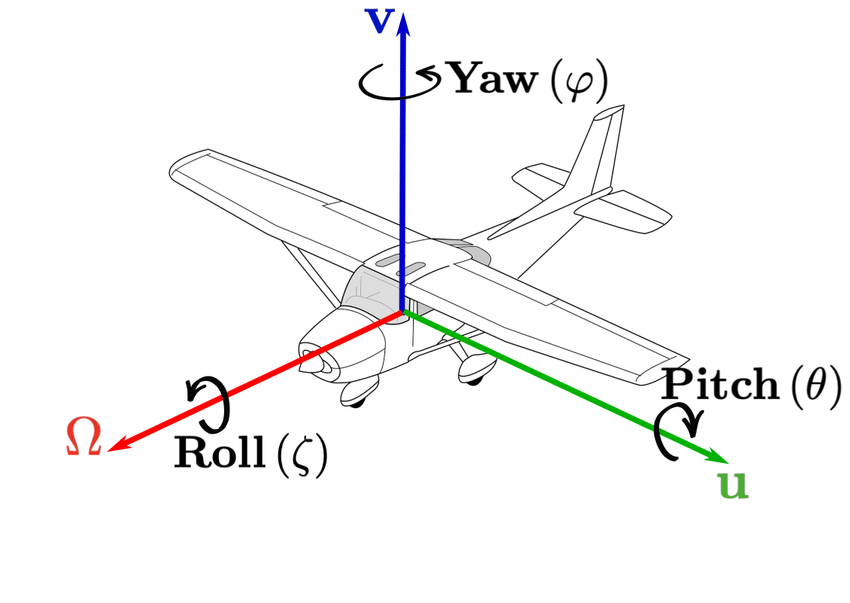
\includegraphics[width=0.5\linewidth]{../ypr.png}
    \caption{ Angles de tangage, de lacet et de roulis d'un avion dont l'orientation du corps est $[\Omega, u, v]$, source \cite{noauthor_figure_nodate}} 
    \label{fig:attitude}

\end{figure}

De nombreuses recherches ont été entreprises pour aborder la question de l'estimation de la pose en utilisant divers types de capteurs et en explorant différentes approches algorithmiques(\ref{subsec: assess_sensor}).\\ 
Dans le cadre de mes recherches, dont l'objectif est de parvenir à une estimation précise de la pose du poignet des nourrissons en se basant sur les données provenant de centrales inertielles et magnétiques (composées d'un accéléromètre triaxial, d'un gyromètre triaxial et d'un magnétomètre triaxial, également appelées IMUs),  \textcite{rihar_caretoy_2016} ont adopté une approche utilisant un filtre de Kalman non linéaire pour fusionner les données d'accéléromètre, de gyromètre et de magnétomètre. Cette fusion de données permet d'estimer l'orientation du poignet du nourrisson, qui est ensuite ajustée en fonction des informations provenant du tapis de pression.\\
En théorie, une simple intégration de l'accélération pourrait nous donner la vitesse, tandis qu'une double intégration nous fournirait des informations sur la position. Cependant, dans la pratique, pour une centrale inertielle standard, la prédiction de trajectoire est applicable sur de très courtes périodes de temps (de l'ordre des secondes) en raison de la non-linéarité, des biais et des bruits présents dans les capteurs de navigation inertielle (IMUs). Cette accumulation d'erreurs se traduit par une erreur de position et d'orientation considérable, à moins d'utiliser d'autres capteurs pour les corriger. Une approche standard consiste à fusionner les données des capteurs inertiels avec celles d'autres capteurs assistés en utilisant des filtres de Kalman ou des filtres complémentaires. Plusieurs schémas de fusion ont été envisagés, tels que la fusion de données provenant du GPS avec les IMUs, des capteurs de pression avec les IMUs, des caméras avec les IMUs, des capteurs de vision stéréo avec les IMUs, et des capteurs de vitesse de fond (DVL) avec les IMUs \cite{noauthor_comparative_2014}. 



\newpage
\section{Expérience}
\label{expé}
\subsection{Extraction de descripteurs}


S'appuyant sur tous les travaux et sur les derniers papiers du projet CareToys \cite{rihar_infant_2019,rihar_caretoy_2016,rihar_infant_2014}, différentes métriques susceptibles de relever un comportement atypique chez les nourrissons ont été répertoriées \ref{tab:metrics} :
\begin{table}[H]
    \centering
    \begin{tabularx}{\textwidth}{|p{0.4\textwidth}|X|}
    \rowcolor{lightgray}
     Partie du corps & Métriques d'évaluation\\
     Avant-bras &  \begin{itemize}
                        \item Accélération;
                        \item Vitesse;
                        \item Position 3D;
                        \item Orientation
                        \item Espace de travail;
                        \item Courbure;
                        \item Longueur de l'arc spectral
                        \item "Jerk"
                        \item La préhension des jouets et l'interaction entre le jouet et la main
                      \end{itemize}
                     \\
\hline
    Tronc & \begin{itemize}
                        \item Centre de pression (COP);
                        \item Amplitude de mouvement de roulement;
                      \end{itemize} \\
\hline
\end{tabularx}
    \caption{Métriques d'évaluation dans le cadre du projet TECH-TOYS}
    \label{tab:metrics}
\end{table}
\subsection{Dataset}
\subsubsection{CareToys dataset}
Les données issues des centrales inertielles, enregistrées au format \textit{hdf5}, comprennent les informations relatives à l'accéléromètre, au gyroscope et au magnétomètre le long des trois axes. Actuellement, elles se trouvent à un stade brut, dépourvues de leurs dimensions physiques, et nécessitent donc un prétraitement ainsi qu'un calibrage. Malheureusement, nous ne disposons pas des données de sensibilité des capteurs, et il n'existe aucune vérité terrain disponible pour les comparer. En conséquence, ces données ne peuvent pas être utilisées pour évaluer la précision et la robustesse de l'algorithme.

Le dispositif Baby-Gym est également équipé de caméras qui enregistrent les mouvements du bébé. Cependant, ces caméras sont mal positionnées, ce qui fait que les enregistrements vidéo disponibles ne montrent qu'une partie de l'interaction. De plus, ils souffrent d'obstructions. Tous ces défauts ont rendu le jeu de données CareToys inutilisable, nous obligeant à créer notre propre ensemble de données afin d'évaluer les performances des algorithmes développés. 
\subsubsection{Dataset émulé}
Les données nécessaires pour évaluer la précision et la robustesse de l'algorithme développé ont été recueillies à l'aide d'une centrale inertielle fixée à une main par le biais d'un smart-phone (voir figure \ref{subfig:phone}). Une interface d'acquisition (voir figure \ref{subfig:apk}) a été utilisée conjointement avec une application mobile appelée \textit{sensor logger}  \cite{choi_awesome_2023}. Les données ont été acquises à une fréquence de 100 Hz, et en parallèle, les mouvements du bras ont été enregistrés à l'aide d'une caméra pour permettre une analyse qualitative de la reconstitution de la pose.\\
Les données collectées comprennent des mesures provenant d'un accéléromètre triaxial, qui enregistre l'accélération le long des trois axes en mètres par seconde carré $(m/s^2)$ tout en corrigeant automatiquement l'effet de la gravité. De plus, un gyroscope triaxial mesure la vitesse angulaire en radians par seconde $(rad/s)$ et calcule l'orientation en utilisant des quaternions ou en radians (comprenant les angles de roulis, de tangage et de lacet) le long des trois axes. Un magnétomètre enregistre l'intensité du champ magnétique en microteslas $(\mu T)$ suivant les trois axes. En outre, d'autres données peuvent être incluses, telles que la position GPS, des images de caméra, des enregistrements audio, des mesures de lumière ambiante, des données de podomètre, etc. Ces données ont été enregistrées en format \textit{csv}.

\begin{figure}[H]
    \begin{subfigure}{0.5\textwidth}
        \centering
        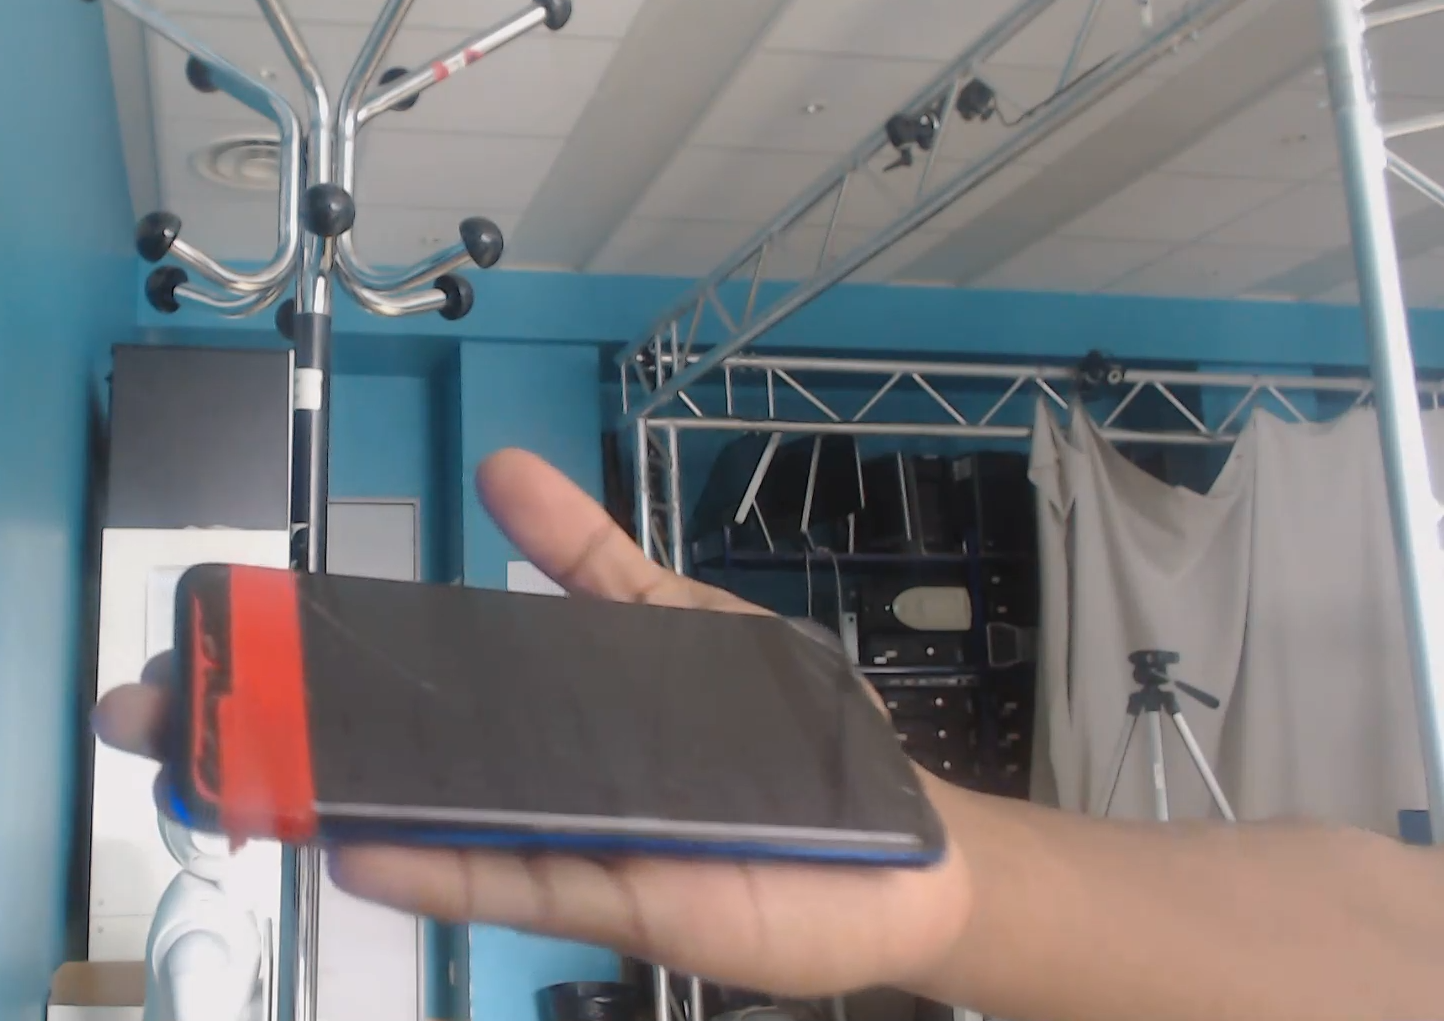
\includegraphics[width=\linewidth]{../phone.png}
        \caption{Smart-phone (IMU)}
        \label{subfig:phone}
    \end{subfigure}
    \begin{subfigure}{0.5\textwidth}
        \centering
        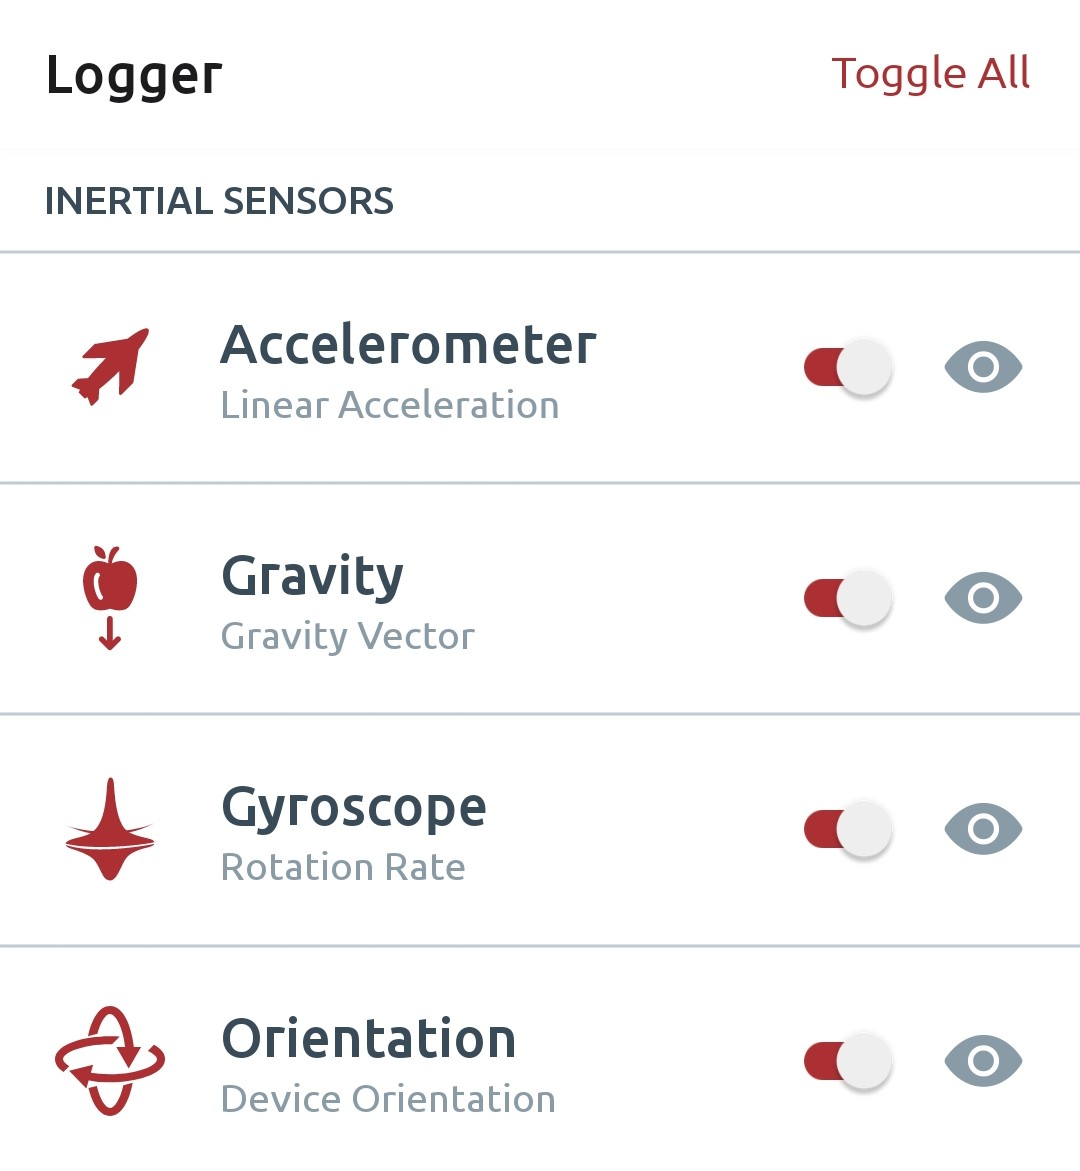
\includegraphics[width=\linewidth, height=7cm]{../apkk.jpg}
        \caption{Interface d'acquisition}
        \label{subfig:apk}
    \end{subfigure}
    \caption{Dispositif d'acquisition des données}
    \label{fig:data}
\end{figure}
\subsection{Résultats}
La précision et la robustesse de l'estimation de l'orientation sont évaluées en utilisant les données fournies par l'application comme référence. Pour effectuer cette évaluation, les données des centrales inertielles sont fusionnées conformément à la méthode décrite dans la section \ref{subsubsec:yrp}. L'algorithme utilisé pour cette fusion des données est \textit{ahrsfilter} de \texttt{Matlab}, disponible depuis la version \texttt{2018b}. Cet algorithme prend en entrée les données des centrales inertielles et renvoie l'orientation sous forme de quaternions ou en fonction des trois axes (en radians). Pour obtenir une estimation plus précise, il est nécessaire de configurer certains paramètres, notamment : "AccelerometerNoise", "GyroscopeNoise", "MagnetometerNoise", "GyroscopeDriftNoise", "LinearAccelerationNoise", "MagneticDisturbanceNoise", "LinearAccelerationDecayFactor" et "MagneticDisturbanceDecayFactor". 

Une évaluation qualitative de l'estimation de l'orientation nous permet de détecter deux paramètres ayant un impact significatif sur la qualité de l'estimation : "MagnetometerNoise" et "LinearAccelerationNoise". 

Une analyse des deux premières secondes du mouvement de la main d'une séquence de six (06) secondes a été capturée (voir \ref{fig:img_mvt}), la reconstruction et l'extraction des descripteurs de la trajectoire de la séquence sont effectuées (voir \ref{subfig:traj_es}, \ref{subfig:workspace_est}), puis nous évaluons l'erreur relative des descripteurs estimés par rapport à ceux de la vérité terrain obtenue à partir de l'orientation donnée par l'application.

On obtient une \textbf{loss1 = 9,04 \%} pour le \textit{Travel Path}, \textbf{11,37 \%} pour la \textit{surface de travail} et \textbf{91,48 \%} pour\textit{le volume de travail} qui est moins robuste en raison des erreurs d'estimation d'orientation créant ainsi des décalages dans le déplacement, ce qui fait varier de manière significative le volume de travail.



\begin{figure}[H]
\begin{subfigure}{1\textwidth}
        \centering
        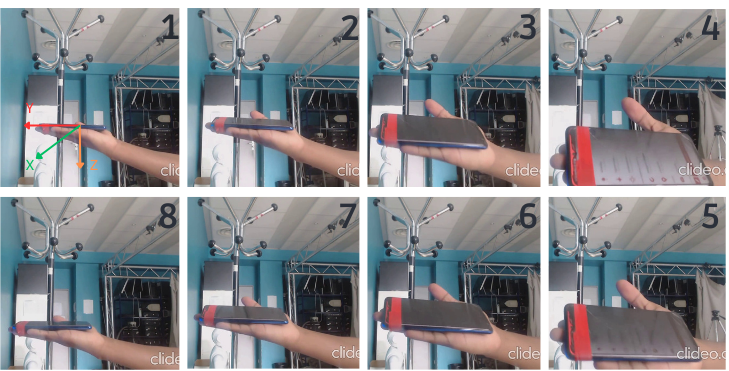
\includegraphics[width=\linewidth, height=8cm]{../results/gt.png}
        \caption{Séquence de mouvement de la main pour l'évaluation qualitative (02 s)}
        \label{fig:img_mvt}
    \end{subfigure}
\begin{subfigure}{0.5\textwidth}
        \centering
        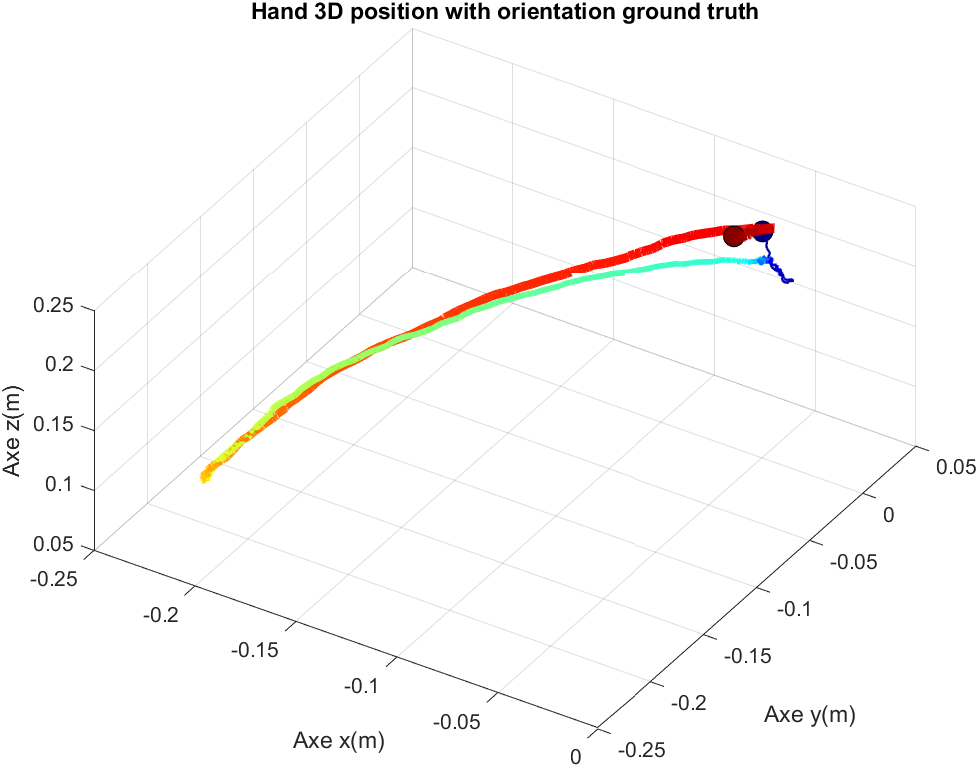
\includegraphics[width=\linewidth]{../results/mvt_1_3d.png}
        \caption{Trajectoire (02 s): vérité terrain }
        \label{subfig:traj_gt}
    \end{subfigure}
    \begin{subfigure}{0.5\textwidth}
        \centering
        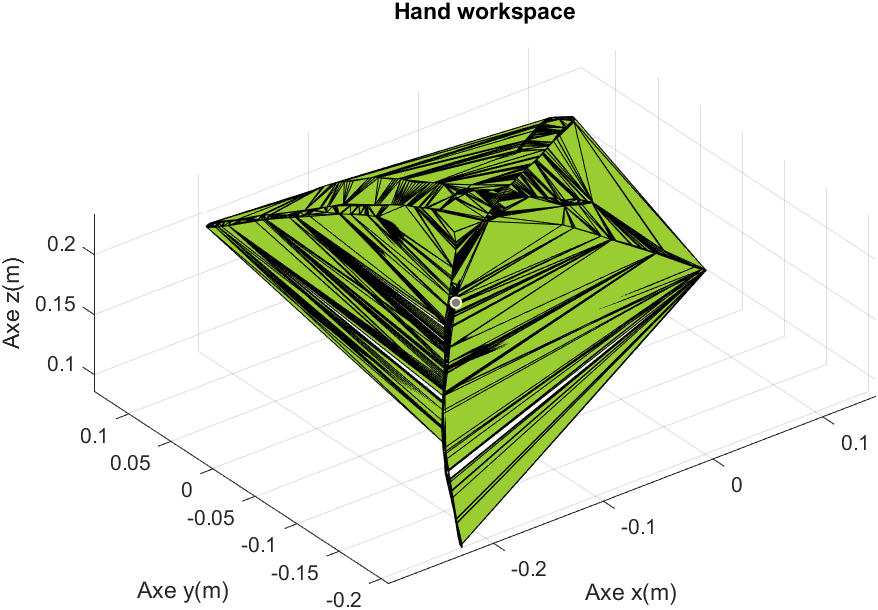
\includegraphics[width=\linewidth, height=7cm]{../results/workspace_ref_min.png}
        \caption{Espace de travail (06 s): vérité terrain}
        \label{subfig:workspace_ref}
    \end{subfigure}

    \begin{subfigure}{0.5\textwidth}
        \centering
        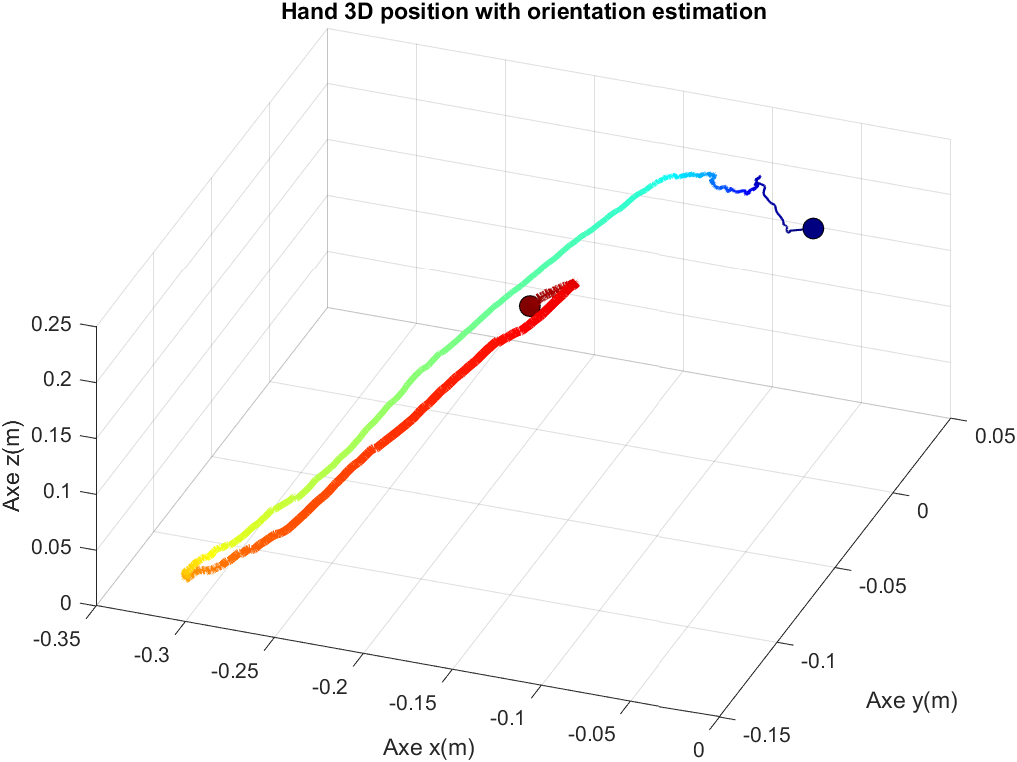
\includegraphics[width=\linewidth]{../results/mvt_1_3d_esmin.png}
        \caption{Trajectoire (02 s): estimation }
        \label{subfig:traj_es}
    \end{subfigure}
    \begin{subfigure}{0.5\textwidth}
        \centering
        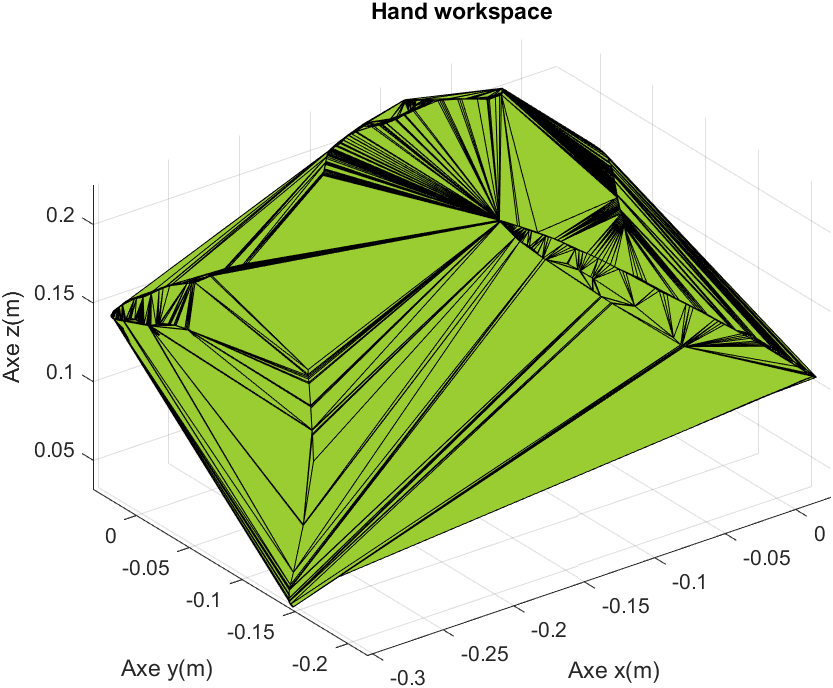
\includegraphics[width=\linewidth, height=7cm]{../results/workspace_est_min.png}
        \caption{Espace de travail (06 s): estimation}
        \label{subfig:workspace_est}
    \end{subfigure}

    \caption{Extraction des descripteurs de trajectoire}
    \label{fig:hand_mvt}
\end{figure}

Par la suite, une optimisation quantitative des paramètres du filtre est envisagée, comme décrit dans \cite{abbeel_discriminative_2005}. Des trajectoires de différentes formes et de finesse variée sont générées dans le but de généraliser les paramètres du filtre. Nous procédons à l'optimisation des paramètres du filtre de Kalman à l'aide de la fonction "tune" de Matlab. Le protocole expérimental se déroule comme suit : \begin{itemize}
    \item \textbf{Sélection de la trajectoire de référence} : Nous débutons le protocole expérimental en choisissant une trajectoire de référence parmi celles générées
        
    \item \textbf{Optimisation du filtre sur la trajectoire de référence} : Un filtre est ensuite ajusté afin d'optimiser son comportement spécifiquement sur cette trajectoire de référence. Cette étape vise à obtenir des paramètres de filtre qui produisent des estimations précises et robustes pour cette trajectoire particulière.
        
    \item \textbf{Création et optimisation de nouveaux filtres pour les trajectoires additionnelles} : Pour chaque trajectoire supplémentaire, un nouveau filtre est créé et ses paramètres sont optimisés spécifiquement sur cette trajectoire. Cette approche permet d'obtenir une "vérité terrain" des descripteurs pour chaque trajectoire, qui servira de référence pour évaluer leur performance.
       
    \item \textbf{Évaluation du filtre optimisé sur d'autres trajectoires} : Après l'optimisation sur la trajectoire de référence, le filtre ainsi obtenu est évalué en utilisant d'autres trajectoires disponibles. Cela permet de déterminer dans quelle mesure les paramètres du filtre optimisé sur une trajectoire donnée généralisent efficacement à d'autres trajectoires.
    
    \item \textbf{Estimation des descripteurs et évaluation de la performance} : Les descripteurs sont ensuite estimés pour chaque trajectoire à l'aide des paramètres du filtre de référence initialement ajusté sur la trajectoire de référence. Ensuite, nous comparons ces descripteurs estimés avec ceux de la vérité terrain à l'aide d'une mesure de perte (loss1). Cette comparaison nous permet de déterminer dans quelle mesure les paramètres du filtre appris sur une trajectoire donnée généralisent sur de nouvelles trajectoires et d'évaluer la robustesse des différents descripteurs associés à l'estimation du filtre de Kalman.
\end{itemize}

\begin{table}[H]
    \centering
    \begin{tabularx}{\textwidth}{|p{0.15\textwidth}|X|X|X|X|X|X|X|X|}
    \rowcolor{lightgray}
        \hline
        Descripteurs | Trajectoires & \cellcolor[HTML]{238CCC} \textbf{Circle slow (Ref)} & Circle fast & Circle shape & Square slow & Square fast & Square shape & Random & Stactic \\ \hline
        \textbf{Travel path} & 0.0 & 0.85 & 0.5516 & 0.2816 & 0.5406 & 0.2377 & 0.3556 & 4.6017 \\ \hline
        \textbf{Surface de travail} & 0.0 & 0.98 & 1.85 & 1.3952 & 3.4701 & 1.2283 & 0.5846 & 1.5e+03 \\ \hline
        \textbf{Volume de travail} & 0.0 & 0.99 & 5.4373 & 4.5307 & 3.9884 & 6.0779 & 0.7416 & 2.97e+05 \\ \hline
        \textbf{Quaternion distance} & 0.0 & 0.63 & 0.308 & 0.2783 & 1.5768 & 1.0941 & 2.9316 & 5 \\ \hline  
    \end{tabularx}
    \caption{loss1 des descripteurs, Trajectoire ref.: 'Circle slow'}
\end{table}
 
 \begin{table}[H]
    \centering
    \begin{tabularx}{\textwidth}{|p{0.15\textwidth}|X|X|X|X|X|X|X|X|}
    \rowcolor{lightgray}
        \hline
        Descripteurs | Trajectoires &  Circle slow & \cellcolor[HTML]{238CCC}\textbf{Circle fast (Ref)} & Circle shape & Square slow & Square fast & Square shape & Random & Stactic \\ \hline
        \textbf{Travel path} & 0.6495 & 0.0 & 0.3140 & 0.8385 & 5.9850 & 3.7829 & 0.1281 & 14.9100 \\ \hline
        \textbf{Surface de travail} & 7.3053 & 0.0 & 1.8787 & 6.1657 & 3.4230 & 4.3260 & 0.6530 & 9.27e+03 \\ \hline
        \textbf{Volume de travail} & 19.2943 & 0.0 & 3.3739 & 11.1143 & 4.9416 & 12.5669 & 0.8756 & 3.18e+07 \\ \hline
        \textbf{Quaternion distance} & 2.5599 & 0.0 & 4.2840 & 4.4080 & 7.3089 & 2.4242 & 4.7059 & 5.8834 \\ \hline  
    \end{tabularx}
        \caption{loss1 des descripteurs, Trajectoire ref.: 'Circle fast'}

\end{table}

\begin{table}[H]
    \centering
    \begin{tabularx}{\textwidth}{|p{0.15\textwidth}|X|X|X|X|X|X|X|X|}
    \rowcolor{lightgray}
        \hline
        Descripteurs | Trajectoires &  Circle slow & Circle fast  & \cellcolor[HTML]{238CCC} \textbf{Circle shape (Ref)} & Square slow & Square fast & Square shape & Random & Stactic \\ \hline
        \textbf{Travel path} & 0.0132 & 0.6513 & 0.0 & 0.3708 & 0.1516 & 0.1294 & 0.4654 & 5.2470 \\ \hline
        \textbf{Surface de travail} & 0.0640 & 0.9434 & 0.0 & 2.1615 & 0.1385 & 0.4834 & 0.6207 & 1.85e+03 \\ \hline
        \textbf{Volume de travail} & 0.2117 & 0.9924 & 0.0 & 6.0408 & 0.2856 & 3.6717 & 0.7805 & 1.72e+05 \\ \hline
        \textbf{Quaternion distance} & 0.0386 & 0.1072 & 0.0 & 3.9363 & 5.2249 & 0.2759 & 3.4326 & 1.9141 \\ \hline  
    \end{tabularx}
        \caption{loss1 des descripteurs, Trajectoire ref.: 'Circle shape'}
\end{table}

\begin{table}[H]
    \centering
    \begin{tabularx}{\textwidth}{|p{0.15\textwidth}|X|X|X|X|X|X|X|X|}
    \rowcolor{lightgray}
        \hline
        Descripteurs | Trajectoires &  Circle slow & Circle fast  &  Circle shape  & \cellcolor[HTML]{238CCC} \textbf{Square slow (Ref)} & Square fast & Square shape & Random & Stactic \\ \hline
        \textbf{Travel path} & 0.0398 & 0.1637 & 1.3071 & 0.0 & 1.0696 & 2.9548 & 0.2592 & 16.0800 \\ \hline
        \textbf{Surface de travail} & 0.4310 & 0.1876 & 8.4584 & 0.0 & 4.8488 & 16.7475 & 2.3805 & 1.22e+04 \\ \hline
        \textbf{Volume de travail} & 0.6323 & 0.5828 & 38.9295 & 0.0 & 10.9859 & 65.1312 & 4.0567 & 5.24e+07 \\ \hline
        \textbf{Quaternion distance} & 0.2819 & 1.3453 & 4.0381 & 0.0 & 5.2690 & 2.3616 & 3.8359 & 5.3946 \\ \hline  
    \end{tabularx}
        \caption{loss1 des descripteurs, Trajectoire ref.: 'Square slow'}
\end{table}

\begin{table}[H]
    \centering
    \begin{tabularx}{\textwidth}{|p{0.15\textwidth}|X|X|X|X|X|X|X|X|}
    \rowcolor{lightgray}
        \hline
        Descripteurs | Trajectoires &  Circle slow & Circle fast  &  Circle shape  & Square slow & \cellcolor[HTML]{238CCC} \textbf{Square fast (Ref)} & Square shape & Random & Stactic \\ \hline
        \textbf{Travel path} & 0.2312 & 0.1120 & 1.6015 & 0.3883 & 0.0 & 5.2366 & 0.1837 & 3.6942 \\ \hline
        \textbf{Surface de travail} & 2.3179 & 0.0071 & 5.0083 & 4.2005 & 0.0 & 71.4706 & 0.0135 & 1.80e+03 \\ \hline
        \textbf{Volume de travail} & 3.8897 & 0.1641 & 13.2986 & 13.0671 & 0.0 & 1.82e+03 & 0.2910 & 3.04e+06 \\ \hline
        \textbf{Quaternion distance} & 1.7006 & 1.1922 & 4.0381 & 4.0685 & 0.0 & 2.0410 & 2.7033 & 3.1562 \\ \hline  
    \end{tabularx}
    \caption{loss1 des descripteurs, Trajectoire ref.: 'Square fast'}
\end{table}

\begin{table}[H]
    \centering
    \begin{tabularx}{\textwidth}{|p{0.15\textwidth}|X|X|X|X|X|X|X|X|}
    \rowcolor{lightgray}
        \hline
        Descripteurs | Trajectoires &  Circle slow & Circle fast  &  Circle shape  & Square slow & Square fast & \cellcolor[HTML]{238CCC} \textbf{Square shape (Ref)} & Random & Stactic \\ \hline
        \textbf{Travel path} & 0.0478 & 0.6382 & 3.8685 & 6.5224 & 3.5830 & 0.0 & 1.0536 & 12.3412 \\ \hline
        \textbf{Surface de travail} & 0.0916 & 0.9297 & 63.1715 & 160.7643 & 57.4153 & 0.0 & 4.653 & 1.06e+04 \\ \hline
        \textbf{Volume de travail} & 0.4186 & 0.9832 & 508.0756 & 2.97e+03 & 200.3426 & 0.0 & 6.7574 & 4.15e+06 \\ \hline
        \textbf{Quaternion distance} & 0.4033 & 1.1897 & 3.5349 & 4.0501 & 6.1521 & 0.0 & 3.0732 & 3.5056 \\ \hline  
    \end{tabularx}
    \caption{loss1 des descripteurs, Trajectoire ref.: 'Square shape'}
\end{table}

\begin{table}[H]
    \centering
    \begin{tabularx}{\textwidth}{|p{0.15\textwidth}|X|X|X|X|X|X|X|X|}
    \rowcolor{lightgray}
        \hline
        Descripteurs | Trajectoires &  Circle slow & Circle fast  &  Circle shape  & Square slow & Square fast & Square shape & \cellcolor[HTML]{238CCC} \textbf{Random (Ref)} & Stactic \\ \hline
        \textbf{Travel path} & 0.1263 & 0.7382 & 1.1276 & 2.8729 & 0.3958 & 2.0800 & 0.0 & 23.7334 \\ \hline
        \textbf{Surface de travail} & 1.7296 & 0.9509 & 4.9131 & 63.7266 & 2.2301 & 21.5410 & 0.0 & 2.84e+04 \\ \hline
        \textbf{Volume de travail} & 2.7177 & 0.9928 & 15.1770 & 263.5282 & 6.4166 & 211.7971 & 0.0 & 8.43e+06 \\ \hline
        \textbf{Quaternion distance} & 1.2682 & 1.4034 & 2.7536 & 3.1484 & 4.2546 & 1.5972 & 0.0 & 3.3200 \\ \hline  
    \end{tabularx}
    \caption{loss1 des descripteurs, Trajectoire ref.: 'Random'}
\end{table}

\begin{table}[H]
    \centering
    \begin{tabularx}{\textwidth}{|p{0.15\textwidth}|X|X|X|X|X|X|X|X|}
    \rowcolor{lightgray}
        \hline
        Descripteurs | Trajectoires &  Circle slow & Circle fast  &  Circle shape  & Square slow & Square fast & Square shape & Random  & \cellcolor[HTML]{238CCC} \textbf{Stactic (Ref)} \\ \hline
        \textbf{Travel path} & 0.7702 & 1.1754 & 15.6564 & 63.9433 & 15.6038 & 10.6502 & 11.4865 & 0.0 \\ \hline
        \textbf{Surface de travail} & 8.3431 & 7.8085 & 232.1026 & 6.3e+03 & 916.6871 & 115.7725 & 108.8398 & 0.0 \\ \hline
        \textbf{Volume de travail} & 24.7350 & 18.2055 & 4.83e+03 & 4.30e+05 & 1.81e+04 & 2.45e+03 & 1.05e+03 & 0.0 \\ \hline
        \textbf{Quaternion distance} & 2.4056 & 2.2300 & 3.6259 & 4.6328 & 7.3611 & 2.2372 & 3.6878 & 0.0 \\ \hline  
    \end{tabularx}
    \caption{loss1 des descripteurs, Trajectoire ref.: 'Stactic'}
\end{table}

Nos constatations soulignent que l'aptitude du filtre de Kalman à généraliser est étroitement liée à la \textit{vitesse et à la trajectoire des mouvements}. Il est intéressant de noter que le filtre semble mieux s'adapter aux trajectoires présentant des vitesses similaires. Cependant, une généralisation satisfaisante des paramètres est également observée sur une gamme variée de trajectoires. Par exemple, pour les trajectoires 'Circle slow', 'Circle fast', et 'Square fast', les erreurs de descripteurs sont minimales lorsqu'elles sont comparées à la trajectoire 'random' (mouvements aléatoires), suggérant que l'optimisation des paramètres du filtre ne se limite pas à une seule trajectoire.

En revanche, une estimation peu fiable des descripteurs est observée pour les mouvements qualifiés de 'statiques', avec des erreurs divergentes. De plus, certains descripteurs se révèlent plus robustes que d'autres. Par exemple, la \textit{'travel path'} et la \textit{'surface de travail'} semblent être des indicateurs plus stables, tandis que d'autres descripteurs comme 'le volume de travail' et 'la quaternion distance' semblent moins fiables pour caractériser les mouvements.
                 
                         
\newpage
\section{Limites}
\label{limites}
Cette section aborde les limitations rencontrées lors de l'estimation des descripteurs de mouvements, ainsi que les approches choisies et les données utilisées. Dans le processus d'estimation des descripteurs de mouvements, deux phases distinctes sont impliquées. Tout d'abord, nous effectuons l'estimation de l'orientation de la main à partir des données d'IMU à l'aide d'un filtre de Kalman. Une première problématique réside dans l'estimation des bruits provenant des gyroscopes et des accéléromètres des centrales inertielles. De plus, l'algorithme implémenté dans \texttt{Matlab} pour le filtre de Kalman est relativement opaque, ce qui limite notre capacité à ajuster et optimiser ses paramètres.

La deuxième étape concerne l'estimation de la position à partir de l'orientation estimée. Cette étape prend en considération plusieurs hypothèses, telles que les mouvements du bras de l'enfant étant généralement effectués bras tendu, et que les mouvements sont de faible amplitude et relativement lents. Cependant, ces hypothèses peuvent introduire des biais significatifs lors de l'application de l'algorithme à des données réelles. Il est important de souligner que nos tests ont été effectués sur des mouvements de personnes adultes, ce qui peut également influencer les performances de l'algorithme lorsqu'il est appliqué à des mouvements d'enfants, qui présentent des caractéristiques motrices différentes. 
\newpage
\section{Conclusion}
Au cours de ce stage nous avons  focalisé notre attention sur l'extraction des descripteurs moteurs à partir des données de trajectoires, en utilisant le filtre de Kalman comme outil principal. À travers notre étude, nous avons souligné l'importance de développer des méthodes d'évaluation robustes et précises pour identifier les marqueurs des TNDs, permettant ainsi une intervention précoce et ciblée. L'utilisation du filtre de Kalman étendu s'est avérée prometteuse pour estimer ces marqueurs de motricité. Nos résultats soulignent l'importance de poursuivre les recherches dans ce domaine crucial. 

Malgré les avancées obtenues, des défis subsistent, notamment en ce qui concerne la gestion des incertitudes liées à l'estimation et la nécessité d'utiliser un jeu de données cohérent, incluant les unités de mesure des capteurs et tenant compte des différentes erreurs de mesures. Pour améliorer la robustesse des méthodes d'analyse, il serait pertinent d'explorer de nouvelles approches, telles que la fusion des données des centrales inertielles avec celles des caméras, comme suggéré par \textcite{ouss_developmental_2018}.
\newpage
\printbibliography
\newpage

\end{document}
